%%%%%%%%%%%%%%%%%%%%%%%%%%%%%%%%%%%%%%%%%%%%%%%%%%%%%%%%%%%%%%%%%%%%%%%%%%%%%%%%
%2345678901234567890123456789012345678901234567890123456789012345678901234567890
%        1         2         3         4         5         6         7         8

\documentclass[letterpaper, 10 pt, conference]{ieeeconf}  % Comment this line out if you need a4paper

%\documentclass[a4paper, 10pt, conference]{ieeeconf}      % Use this line for a4 paper

\IEEEoverridecommandlockouts                              % This command is only needed if 
                                                          % you want to use the \thanks command

\overrideIEEEmargins                                      % Needed to meet printer requirements.

% See the \addtolength command later in the file to balance the column lengths
% on the last page of the document

% The following packages can be found on http:\\www.ctan.org
\usepackage{graphicx} % for pdf, bitmapped graphics files
%\usepackage{epsfig} % for postscript graphics files
%\usepackage{mathptmx} % assumes new font selection scheme installed
%\usepackage{times} % assumes new font selection scheme installed
\usepackage{amsmath} % assumes amsmath package installed
\usepackage{amssymb}  % assumes amsmath package installed
\usepackage{color}
\usepackage[]{algorithm2ea}
\usepackage{caption}
\usepackage{subcaption}




\newcommand{\dhm}[1]{\textcolor{blue}{Dylan: #1}}


\title{\LARGE \bf
Bootstrapping Trajectory Transfer from Multiple Demonstrations with Applications to Deformable Object Manipulation
}

\author{Ankush Gupta, Dylan Hadfield-Menell, Robbie Gleichman, and Pieter Abbeel$^{1}$% <-this % stops a space
\thanks{Department of Electrical Engineering and Computer Sciences, University of California at Berkeley, CA, USA.
  {\tt\small gupta, dhm, rgleichman, pabbeel} @berkeley.edu}}

\DeclareMathOperator*{\argmin}{arg\,min}

\begin{document}

\RestyleAlgo{boxruled}

\maketitle
\thispagestyle{empty}
\pagestyle{empty}


%%%%%%%%%%%%%%%%%%%%%%%%%%%%%%%%%%%%%%%%%%%%%%%%%%%%%%%%%%%%%%%%%%%%%%%%%%%%%%%%
\begin{abstract}
Deformable object manipulation remains a challenging task in robotics.
Continuous, high dimensional, state and action spaces make standard
model-based approaches to manipulation planning intractable. Recent work
has shown progress on this task by learning from
demonstrations through 
\emph{trajectory transfer}~\cite{Schulmanetal_ISRR2013, Schulmanetal_IROS2013}. This approach avoids planning in the state space of a deformable object
by finding a spatial warping that can be used to apply an expert demonstration
to a new scene.

We propose a method for improving trajectory transfer that makes use of bootstrapping examples through simulation. Given a simulator and a way to detect success, we augment our trajectory library with example states and transferred trajectories that have succeeded in simulation. We apply this approach to a simulated overhand knot-tying task. The approach described in Schulman et al.~\cite{Schulmanetal_ISRR2013} achieves a success rate of 59\%. We demonstrate performance of up to 85\%. 

\end{abstract}


%%%%%%%%%%%%%%%%%%%%%%%%%%%%%%%%%%%%%%%%%%%%%%%%%%%%%%%%%%%%%%%%%%%%%%%%%%%%%%%%
\section{INTRODUCTION}
A large challenge in applying standard manipulation and planning techniques to
deformable object manipulation is that of tractable modelling. Deformable object 
are often characterized by high-dimensional, continuous state-action spaces. Model-based 
planning has yet to scale up to the task of efficient planning in this
setting.

Recent work have gained traction on this problem through the technique of 
learning from demonstrations~\cite{Schulmanetal_ISRR2013,Schulmanetal_IROS2013}.
These results are achieved through \emph{trajectory transfer}, where a demonstration
trajectory is generalized to fit to a new scenario. Trajectory transfer finds a non-rigid
registration between an example scene and the current scene that trades off between
goodenss-of-fit and the curvature of the registration. 
This method of transfer is model-free and obviates the need to plan in typically
intractable models of deformable objects. Trajectory transfer has demonstrated 
state-of-the-art performance for knot-tying and suturing.

An important aspect of this strategies is incorporation of multiple demonstrations. 
By increasing the number of demonstrations, it becomes possible to do more
tasks. Additionally, demonstrations can take the form of steps in a task and can be
ordered and combined to further increase the set of possible successful manipulations.

However, a key problem remains: how should we pick which trajectory to transfer
from a library of options given an input scene? Incorrect selection may lead us
to fail at a task which would otherwise be possible for the correct selection of 
trajectories. Furthermore, how can we use experience to improve trajectory transfer 
both at the level of selecting a trajectory to transfer and at the level of transferring
a single trajectory.

In this paper we present a method for improving the performance associated with
a library of demonstrated trajectories through simulated attempts at trajectory
transfer and feedback about the success of those transferred trajectory. Our approach
applies bootstrapping improve on standard trajectory transfer by 
by treating successful transfers as new demonstrations. This enables us improve
performance without requiring new human supervision. Treating successful simulations
as new demonstrations builds up a higher granularity representation of states where
we expect transfer to succeed and enables better selection of a trajectory to 
generalize at test time. In addition, the feedback recieved can improve our ability
to transfer a single trajectory by building an implicit model of non-rigid 
deformations such that transfer succeeds. We demonstrate the effectiveness 
of these improvements in knot-tying task and find improvements  
of up to 25\% over the transfer method described in Schulman et al.~\cite{Schulmanetal_ISRR2013}.

\begin{figure}
  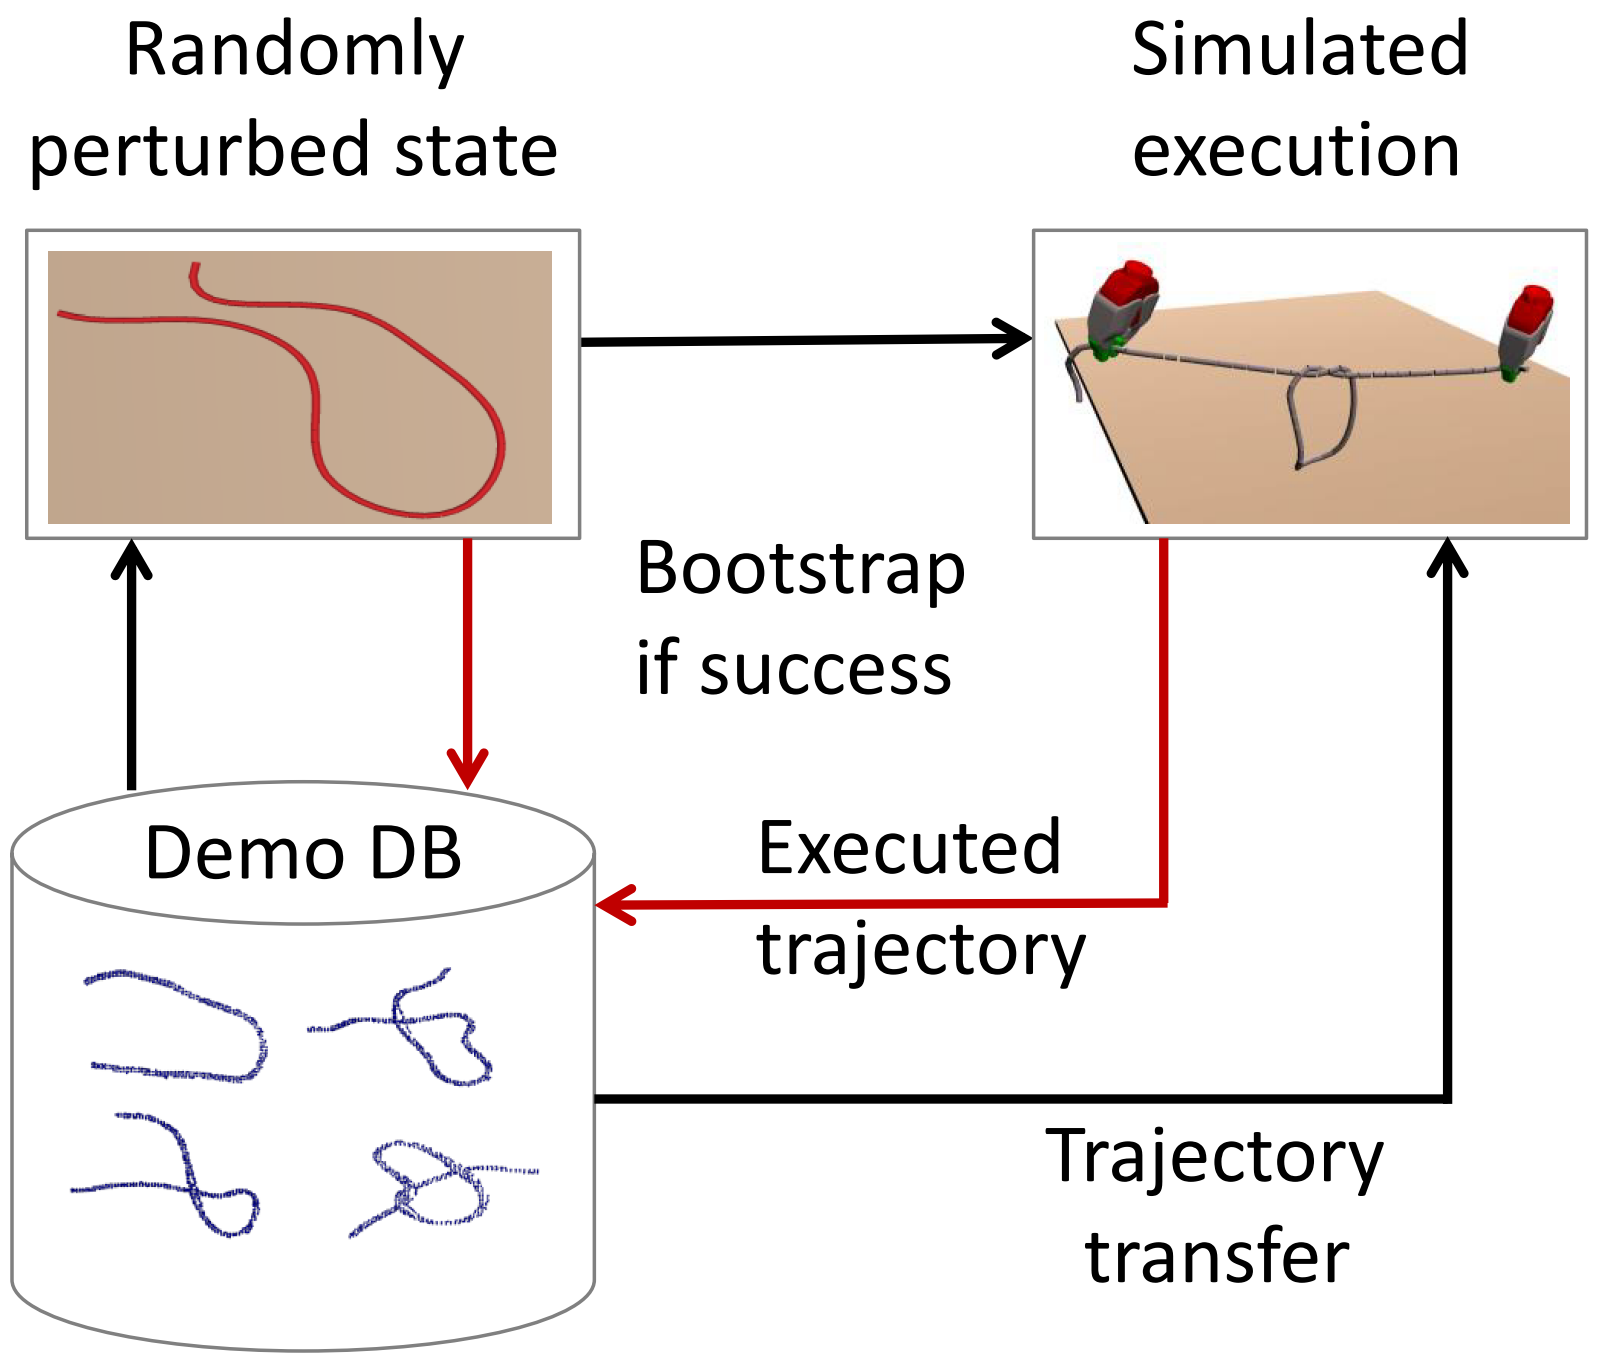
\includegraphics[width=\linewidth]{figs/teaser.png}
  \caption{Diagram of the bootstrapping approach we employ. Our system uses simulation
           of perturbed states from our demonstration set to augment a library of expert
           demonstrations. We find that this approach can leverage synthetic data to improve
           on the applicable of expert demonstrations by better modelling of states that
           trajectories can transfer to and allowing our approach to penalize less for
           transformations where transfer succeeds.}
  \label{fig:knot_steps}
\end{figure}





\section{Related Work}
Our approach to learning from demonstrations avoids building explicit representations
and models of objects and states spaces. Thus, it is well suited to deformable object 
manipulations. It is challenging to manipulate deformable objects due to their nonlinearity
and because the configuration spaces of such objects may be
infinite-dimensional~\cite{Lamiraux_IJRR2001}.

In previous work, Wada et al. model textile fabric and sponge blocks
coarsely and then apply a control method that is robust
to discrepancies between the coarse model and the
object~\cite{Wada_ArticMotion2000}. Howard et al. present a more
general approach for grasping 3D deformable objects
that does not assume prior knowledge of the object.
They model particle motion of the object using nonlinear partial differential
equations, and train a neural network for determining the minimum force
required for manipulating the object~\cite{Howard_AutRobots2000}.

We validate our approach and present results for knot tying. There is
a rich literature of knot-specifc approachs to this problem.
For instance, in knot planning from observation (KPO), knot theory is used
to recognize rope configurations and define
movement primitives from visual observations of humans tying
knots~\cite{Morita_ICRA2003, Takamatsu_TransRob2006}.
Existing motion planning approaches for knot tying use topological
representations of rope states (i.e. sequences of rope crossings and their
properties) and define a model for transitioning between topological
states~\cite{Moll_IEEERobot2006, Saha_ExpRobotics2008, Wakamatsu_IJRR2006}.
Robust open loop execution of knot tying has also been explored~\cite{Bell_PhD2010}

The problem of learning from demonstrations (LfD) deals with the generalization of expert demonstrations to 
new scenarios~\cite{Argall_2009, Schaal_1999}. Behavioral cloning is an approach to LfD that 
directly learns a policy to mimic an expert's behavior.

One of the first successful applications of this strategy is the ALVINN system~\cite{Pomerleau_NIPS1989}, which utilizes a 
neural network to learn a steering policy that enables an autonomous car to follow a road.
\cite{muller2005off} use a convolutional network to learn a steering policy for off-road driving.
\cite{Ratliff_Humanoids2007} uses multi-class classification to learn a function that scores actions 
to predict good foot steps for robot locomotion and good grasps for robot manipulation.
\cite{Ross_2013} propose a method to directly control a Micro UAV from RGB camera input.

Miyamoto et al. describe an approach for learning to play Kendama~\cite{Miyamoto_1996} and hit a 
tennis ball~\cite{Miyamoto_1998} from demonstrated actions. 
Their method is successful at generalizing human trajectories and incorporates sequential information 
from multiple demonstrations.
However, this approach requires hand tuning of waypoints and does not generalize to new scenes.

Isaac et al.~\cite{Isaac_ICML2003} use behavioral cloning to learn to fly an airplane, by making use of an abstract, 
goal-directed, layer which sits on top of a low-level PID controller.
This goal-directed learning is similar in spirit to ours, although it makes use of a different formalism
and uses simpler low level controllers.

Calinon et al. learn a mixture of Gaussians to represent the joint trajectory of the robot and environment
state across multiple demonstrations, and infer the trajectory for a new
environment state by conditioning on that state~\cite{Calinon_SMC2007, Calinon_HUM2009}. Their approach
assumes access to a feature representation of the environment, so it cannot directly be applied to tasks in
environments without fixed feature representations --- such as our application of knot tying.


\section{Trajectory Transfer with Thin Plate Splines}
\emph{Trajectory transfer} is an approach to learning from expert demonstrations~\cite{Schulmanetal_ISRR2013}. The trajectory transfer
algorithm is given a current scene, $s_{test}$, demonstration scene, $s_{demo}$ and a demonstration trajectory,  
$t_{demo}$, as input. We assume that the scenes are made up of matched points in $\mathbb{R}^3$. The first step is to 
find a function, $f^*:\mathbb{R}^3 \rightarrow \mathbb{R}^3$, as the solution to the following optimization problem:
\begin{equation}\min_f \sum_i ||s_{test}^{(i)} - f(s_{demo}^{(i)})||^2 + C\int dx ||D^2(f)||^2_{Frob}.\label{eq:tps}\end{equation}
The minimizing $f$ will be a Thin Plate Spline, and can be expressed as a linear combination of basis
functions about the correspondence points~\cite{Wahba_TPS1990}. $C$ is a hyper-parameter that trades off
between goodness of fit and the curvature of the function. The solution to this optimization can be computed
as the solution to a linear system of equations.

Given a warping, $f^*$, between the demo and test scenes, we take each pose from the demo trajectory and pase it through
$f^*$. Poses are transferred by mapping coordinate frames through the jacobian of $f^*$. The trajectory that results from this
is used to guide a motion planner that finds a similar feasible trajectory. This trajectory is executed in the test scene.
In the case where correspondences are not known initially, one can use TPS-RPM, an approach that jointly finds
correspondences and a mapping between them by alternating between estimating correspondences and solving for 
a thin plate spline\cite{Chui_CVIU2003}.

Schulman et al.~\cite{Schulmanetal_ISRR2013} provide some intuition for scenarios where this approach is likely
to succeed. They assume a cost function, $L$, on states and trajectories, a reasonable option might be 0-1 loss, depending
on whether the trajectory successfully executes a desired manipulation in a given state.  Then we can justify warping the
state $s$ and the trajectory $t$ 
in the case where $L(s, t)~=~L(f(s), f(t))$. Essentially, the of a manipulation is preserved under a class of transformations,
thus, we can successfully transform a state and trajectory and maintain the relation that the manipulation succeeds. The set of functions
that have this property define a set of states that a particular demonstration trajectory can transfer to.

A final aspect of this approach is the incorporation of multiple trajectories. Given a library of trajectories,
one can increase the number of states that can be generalized to. This allows an expert to demonstrate steps of a complex task
which can be sequenced at test time. This can make trajectory transfer more robust and reliable, as an expert can also
include demonstrations to recover from common failures. Current approaches use the nearest-neighbor with respect to registration
cost (the value of the optimization problem defined in (\ref{eq:tps})). This corresponds to modeling the set of states a demonstration
can generalize to---that is states for which $L$ is invariant to the TPS warping found by TPS-RPM---as a hyper-sphere 
in a high-dimensional space where this registration cost is a distance function.




\section{Bootstrapping New Demonstrations from Experience}
In this section, we present our algorithm for bootstrapping new examples 
from expert demonstrations. At its core, the idea is simple: if we get
examples of new states that are able to successfully transfer a trajectory to,
we get a new example of a successful manipulation. We can use these examples
to transfer trajectories better in new settings.

\subsection{Modeling Transfer Sets}
Formally, we assume access to an environment and a reward signal. In our work, this
environment is a simulated although in the approach can apply to real settings. 
Our reward signal is a 1-0 response which tells us if a manipulation succeeds. For 
tasks involving several steps, we associate success with a manipulation if a success
signal is received before a fixed time horizon is reached.

To ease discussion, we introduce the concept of a \emph{transfer set}. Given a method for
transferring a demonstration trajectory to a new state, the associated transfer set is
the set of states such that the transferred trajectory will successfully execute the
demonstrated manipulation. With this terminology, we can consider the nearest-neighbor
selection method from Schulman et al.~\cite{Schulmanetal_ISRR2013} as approximating the
transfer set for a particular demonstration with a hyper-sphere defined with respect
to the registration cost.

A first step to improving the selection step is to build a richer
model of the transfer set associated with a trajectory. Given a set of
states that a trajectory, $t$,  has been successfully transferred to, $S_T$, we can
model a transfer set with a collection of hyper-spheres around those states.
Then, when it comes time to select a trajectory to generalize, we pick according to
the following rule:
\begin{equation}
\underset{t}{\argmin} \ \ \underset{s\in S_t}{\min} \ \ {\text registration\_cost}(s).
\end{equation}
Alg.~\ref{alg:trans-set} illustrates a greedy algorithm for building up the sets $S_t$ given
access to a simulation environment and a reward signal. 

\subsection{Bootstrapping New Examples}
Building a better model of the transfer set for a trajectory provides a way
to better select trajectories. However, it discards a reasonable amount of
data. During execution, have access to the transferred trajectories in addition
to the states they were transferred to. In some sense, these are new examples of 
successful manipulations in their own right. Instead of simply storing
the states we successfully transfer to, we can add those examples to our trajectory 
library and consider transferring the derived trajectories to new scenes. 
Alg.~\ref{alg:bootstrap} shows a greedy method for building a bootstrapped trajectory
library from experience.

\begin{algorithm}[H]
 \SetKwInOut{originalDemos}{input}\SetKwInOut{bootstrappedDemos}{output}

 \originalDemos{originalDemos $= \left[(s_{demo1},t_{demo1}), (s_{demo2}, t_{demo2}), \ldots \right]$}
 \bootstrappedDemos{bootstrappedDemos, the bootstrapped trajectory library}
 bootstrappedDemos $\leftarrow$ originalDemos\;
  \For{$i \leftarrow 0$ \KwTo $N$}{
        $s_{test}$ $\leftarrow$ sample\_from\_test\_distribution()\;
        $(s_{parent}, t_{parent})$ $\leftarrow \underset{(s,t) \in bootstrappedDemos}{\argmin} registration\_cost(s, s_{test})$\;
        $t_{warped}$ $\leftarrow$ $apply\_TPS\_RPM\_transform(s_{parent}, s_{test}, t_{parent})$\;

        successful\_trajectory\_execution $\leftarrow$ $executeTrajectory(t_{warped})$\;
        \If{successful\_trajectory\_execution}{
          bootstrappedDemos $\leftarrow$ $(s_{parent}, t_{parent})$ $\cup$ bootstrappedDemos \;
        }
    }
 \caption{Bootstrapping a Trajectory Library}
 \label{alg:bootstrap}
\end{algorithm}

One possible objection to this method is as follows: given that these derived examples
simply deformations of an original, why would we expect this to be better than simply
transferring the original? The answer to this question is based in different
aspects of the TPS approach to trajectory transfer.

The first is that, in addition to finding a transfer function that minimizes curvature,
we are also finding correspondences between points in the different scenes. Finding 
correspondences is a difficult and well-studied problem in computer vision and the best
approaches are subject to local optima. The TPS-RPM algorithm is no exception. 

We could appeal to local features to improve this difficulty, but finding feature descriptors 
that capture important aspects of general manipulation problems is a difficult task. The
states we add to our trajectory library are examples of states and correspondences that 
successfully transferred a demonstration trajectory. By transferring directly from those
states, as opposed to the original demonstration state, we are providing a better 
initialization to the TPS-RPM algorithm and we should be able to find better correspondences
between points.

The second reason we would expect this to be successful is that in transferring derived
states and trajectories, the we enable the use of a broader class of functions for 
transferring trajectories. In transferring a trajectory, $t$, from state $s_1$ through
state $s_2$ to $s_3$, we compute a thin plate spline from $s_1$ to $s_2$ 
($f_{1\rightarrow 2}$) then from $s_2$ to $s_3$ ($f_{2\rightarrow 3}$). The trajectory we
execute is then $f_{1\rightarrow 2}(f_{2\rightarrow 3}(t)) \ne f_{1\rightarrow 3}(t)$. 
Instead of using a thin plate spline, we are using a form of iterated thin plate spline.

The intuition behind this is that a thin plate spline represents an encoding of a preference
for non-rigid functions to transfer a state. For a general approach, this is a good
preference to have. However, for a particular manipulation task, not all deformations
will have the same effect on transfer success. 

As an example, consider a robot transferring
trajectories for opening a drawer. In transferring the first portion of a demonstration,
almost any deformation is OK: all that needs to happen is that the robot grabs the drawer handle.
However, for the second part---actually opening the drawer---almost any non-rigid deformation
will result in a failed transfer.

In fitting a thin plate spline to derived trajectories, we gain the ability 
to learn these transfer properties for the manipulation we are exploring.
The non-rigid deformations that resulted in successful transfers are no longer
penalized in fitting the thin plate spline. For our drawer example, after enough
examples of successful transfers this technique would effectively learn to allow
certain types of deformations (e.g. those that allow us to grab the drawer) but still
maintain the ability to penalize for others (e.g. deformations that don't allow the robot to
open the drawer).




\section{Experiments and Results}
\subsection{Experimental Setup}
We evaluate our 2 learning method in a simulation environment on an overhand knot-tying task.
We use floating gripper with joint constraints to study the effects of trajectory transfer
without the complications of altering derived trajectories to incorporate joint constraints.

\subsubsection{Demonstrations}
The demonstrations we use to initialize the trajectory library are those used by
Schulman et al.~\cite{Schulmanetal_ISRR2013} for their experiments. The demonstrations
split the task of tying an overhand knot into 3 steps. Demonstrations were collected
by physically guiding a Willow Garage PR2 through these steps and opening or closing 
the grippers at the appropriate points. There are 36 demonstrations of full knot ties
in the data set in addition to several demonstrations that correct for common failures.
Point clouds were collected with a Kinect RGBD camera and filtered by color to extract
rope points. 

\begin{figure}
  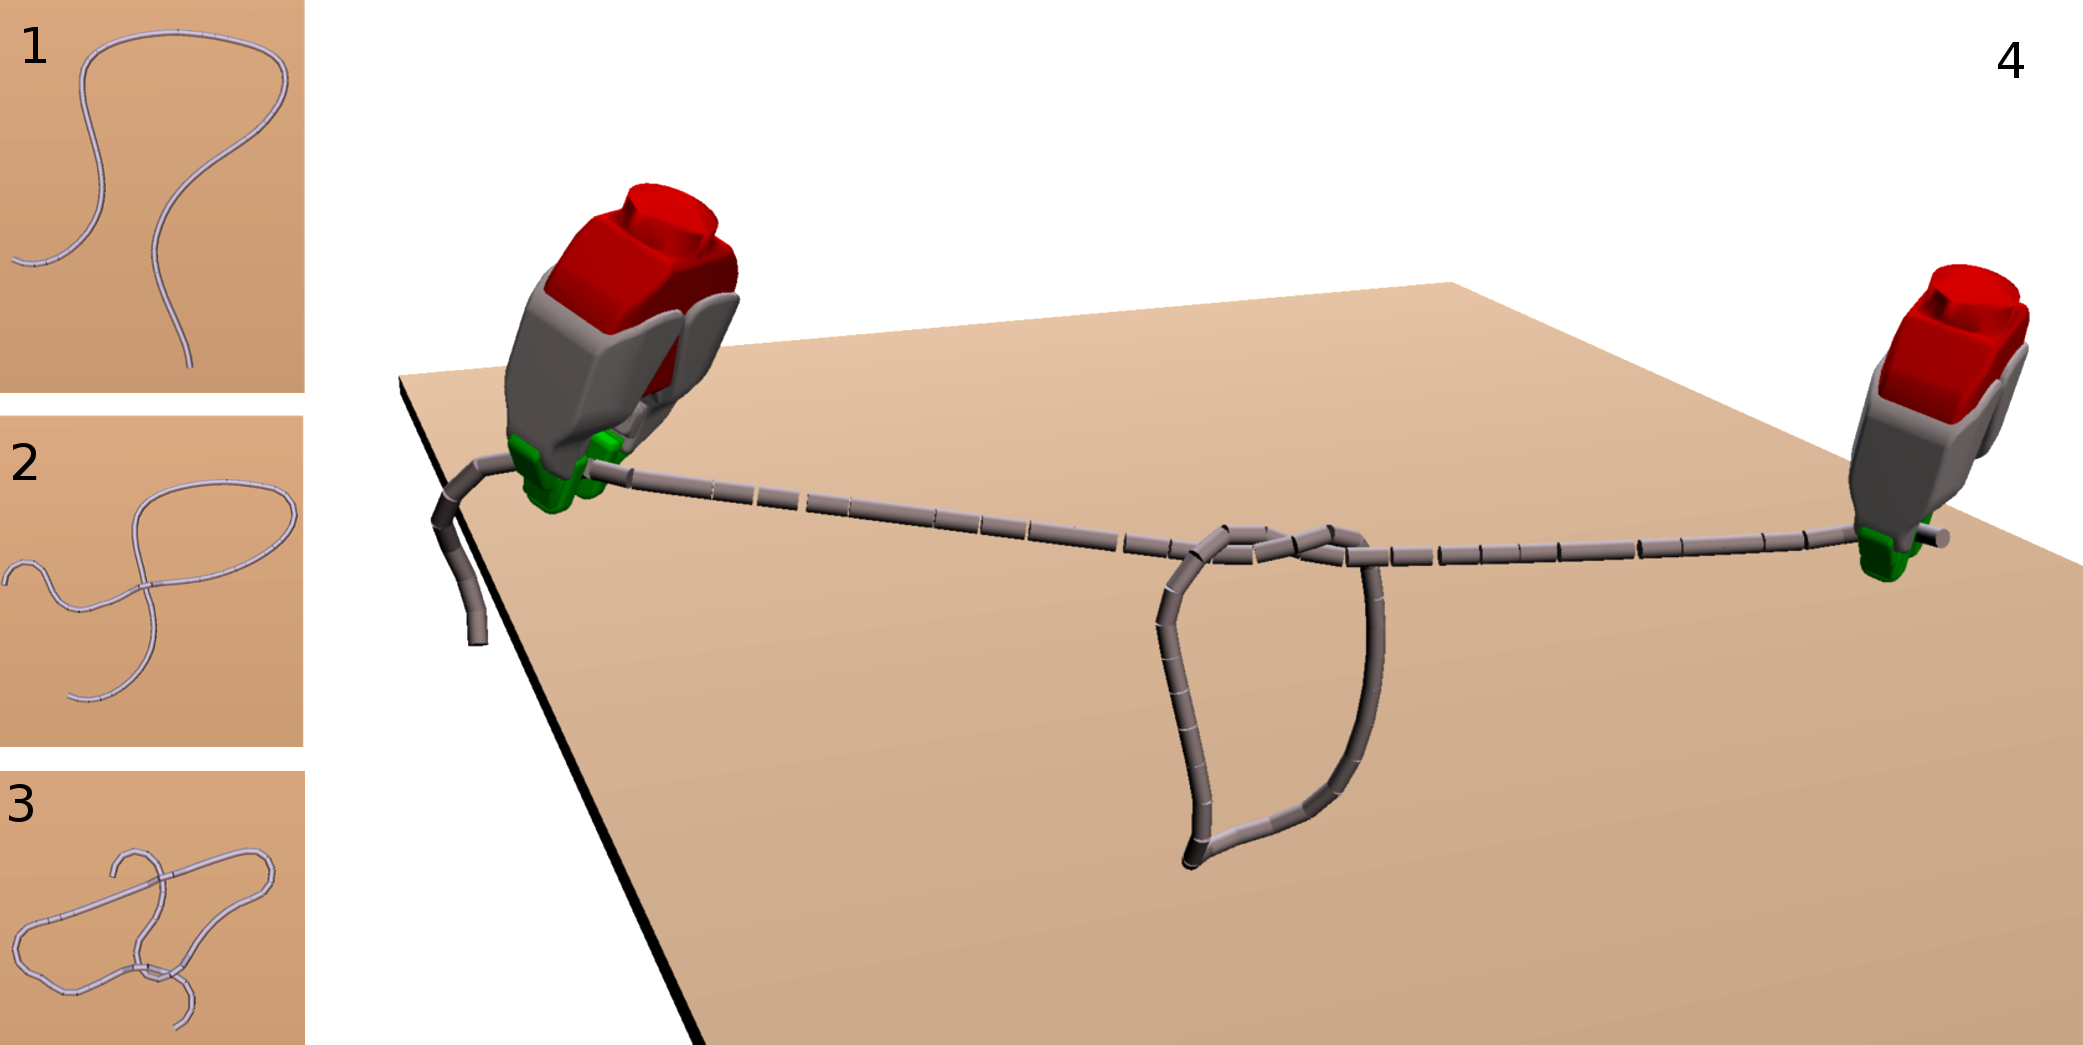
\includegraphics[width=\linewidth]{figs/cov.png}
  \caption{Example of the steps involved in an overhand knot-tying task in our simulated
           environment. The strandard demonstrations in our trajectory tie a knot as a 
           sequence of 3 steps.}
  \label{fig:knot_steps}
\end{figure}


\subsubsection{Simulation Environment and Task Distribution} 
The tasks we consider are simulations of an overhand knot tying tasks. 
We simulate a rope as a chain of cylinders linked by bending and torsional constraints.
Simulation is done through the use of Bullet Physics engine~\cite{Bullet_Physics}.

Our distribution over initial states is defined procedurally. We begin by uniformly
selecting an initial state from the demonstration. Then 7 points along the rope are 
drawn and subjected to 10cm of perturbation in a random direction. Finally a random
rotation between 0 and $\frac{pi}{4}$ is applied to the perturbed rope. We ran our
bootstrapping algorithms on initial states from this distribution and tested on a 
separate evaluation set.

\subsubsection{Training and Evaluation}
In order to explore the improvements from better modeling and compare with improvements
that come from better transfer of a particular trajectory, we ran two sets of experiments.
We generated 10 sequences of 170 states drawn IID from our initial state distribution.
We built a modified trajectory library for both approaches on each of the training sequences.
Training was accomplished by an initial exploration phase of 50 attempts where only the initial
demonstrations were used. Then there were 120 knot-tying attempts that chose and transferred
trajectories using the new techniques. We evaluated our bootstrapped libraries on an evaluation
set that consisted of 300 initial states that were held out from training.

\subsection{Results & Analysis}

On our test set, across 10 different training sequences, we our bootstrapped trajectories
yieled an average success rate of 74\%. This represents a 15\% increase over the baseline 
approach which only used the initial human demonstrated trajectories. Our best performing
run gained an additional 10\% to reach an 84\% success rate overall. Fig.~\ref{fig:results} 
illustrates these results.

We believe that these results indicate the utility of this approach to improving
trajectory transfer with non-rigid registration. By successively warping from 
states that we have transferred trajectories successfully, we enable transfer
that penalizes less for deformations that preserve important aspects of the manipulation
task without hand-coding prior knowledge. For example, in our knot-tying task, trajectory 
will transfer robustly for deformations in the X-Y plane, but deformations in the Z dimension
will often cause unsucessful transfers. Fig.~\ref{fig:warps} illustrates this for one
example from our evaluation set. Directly warping with TPS-RPM fails because correspondences 
are hard to find. Even with correct correspondences, standard trajectory transfer is
prone to failure because the thin plate spline fit will penalize equally for all deformations.
By contrast, bootstrapping from successful trajectories discovers this structure
and is able to leverage it to succeed. 

We believe that these results indicate the utility of this approach. We have demonstrated that
given access to feedback about successful transfers can have large payoffs. However,
the particular algorithm we use to actually perform this bootstrapping exhibits large variance.
We believe that this can be combatted through more explicit and careful tradeoff between
exploration and exploitation. After the intial exploration phase, the focus on exploitation
can miss the potential to better transfer new trajectories. A more sophisticated treatement
of the exploration exploitation tradeoff in this setting is an important direction for future work.

\begin{figure}
  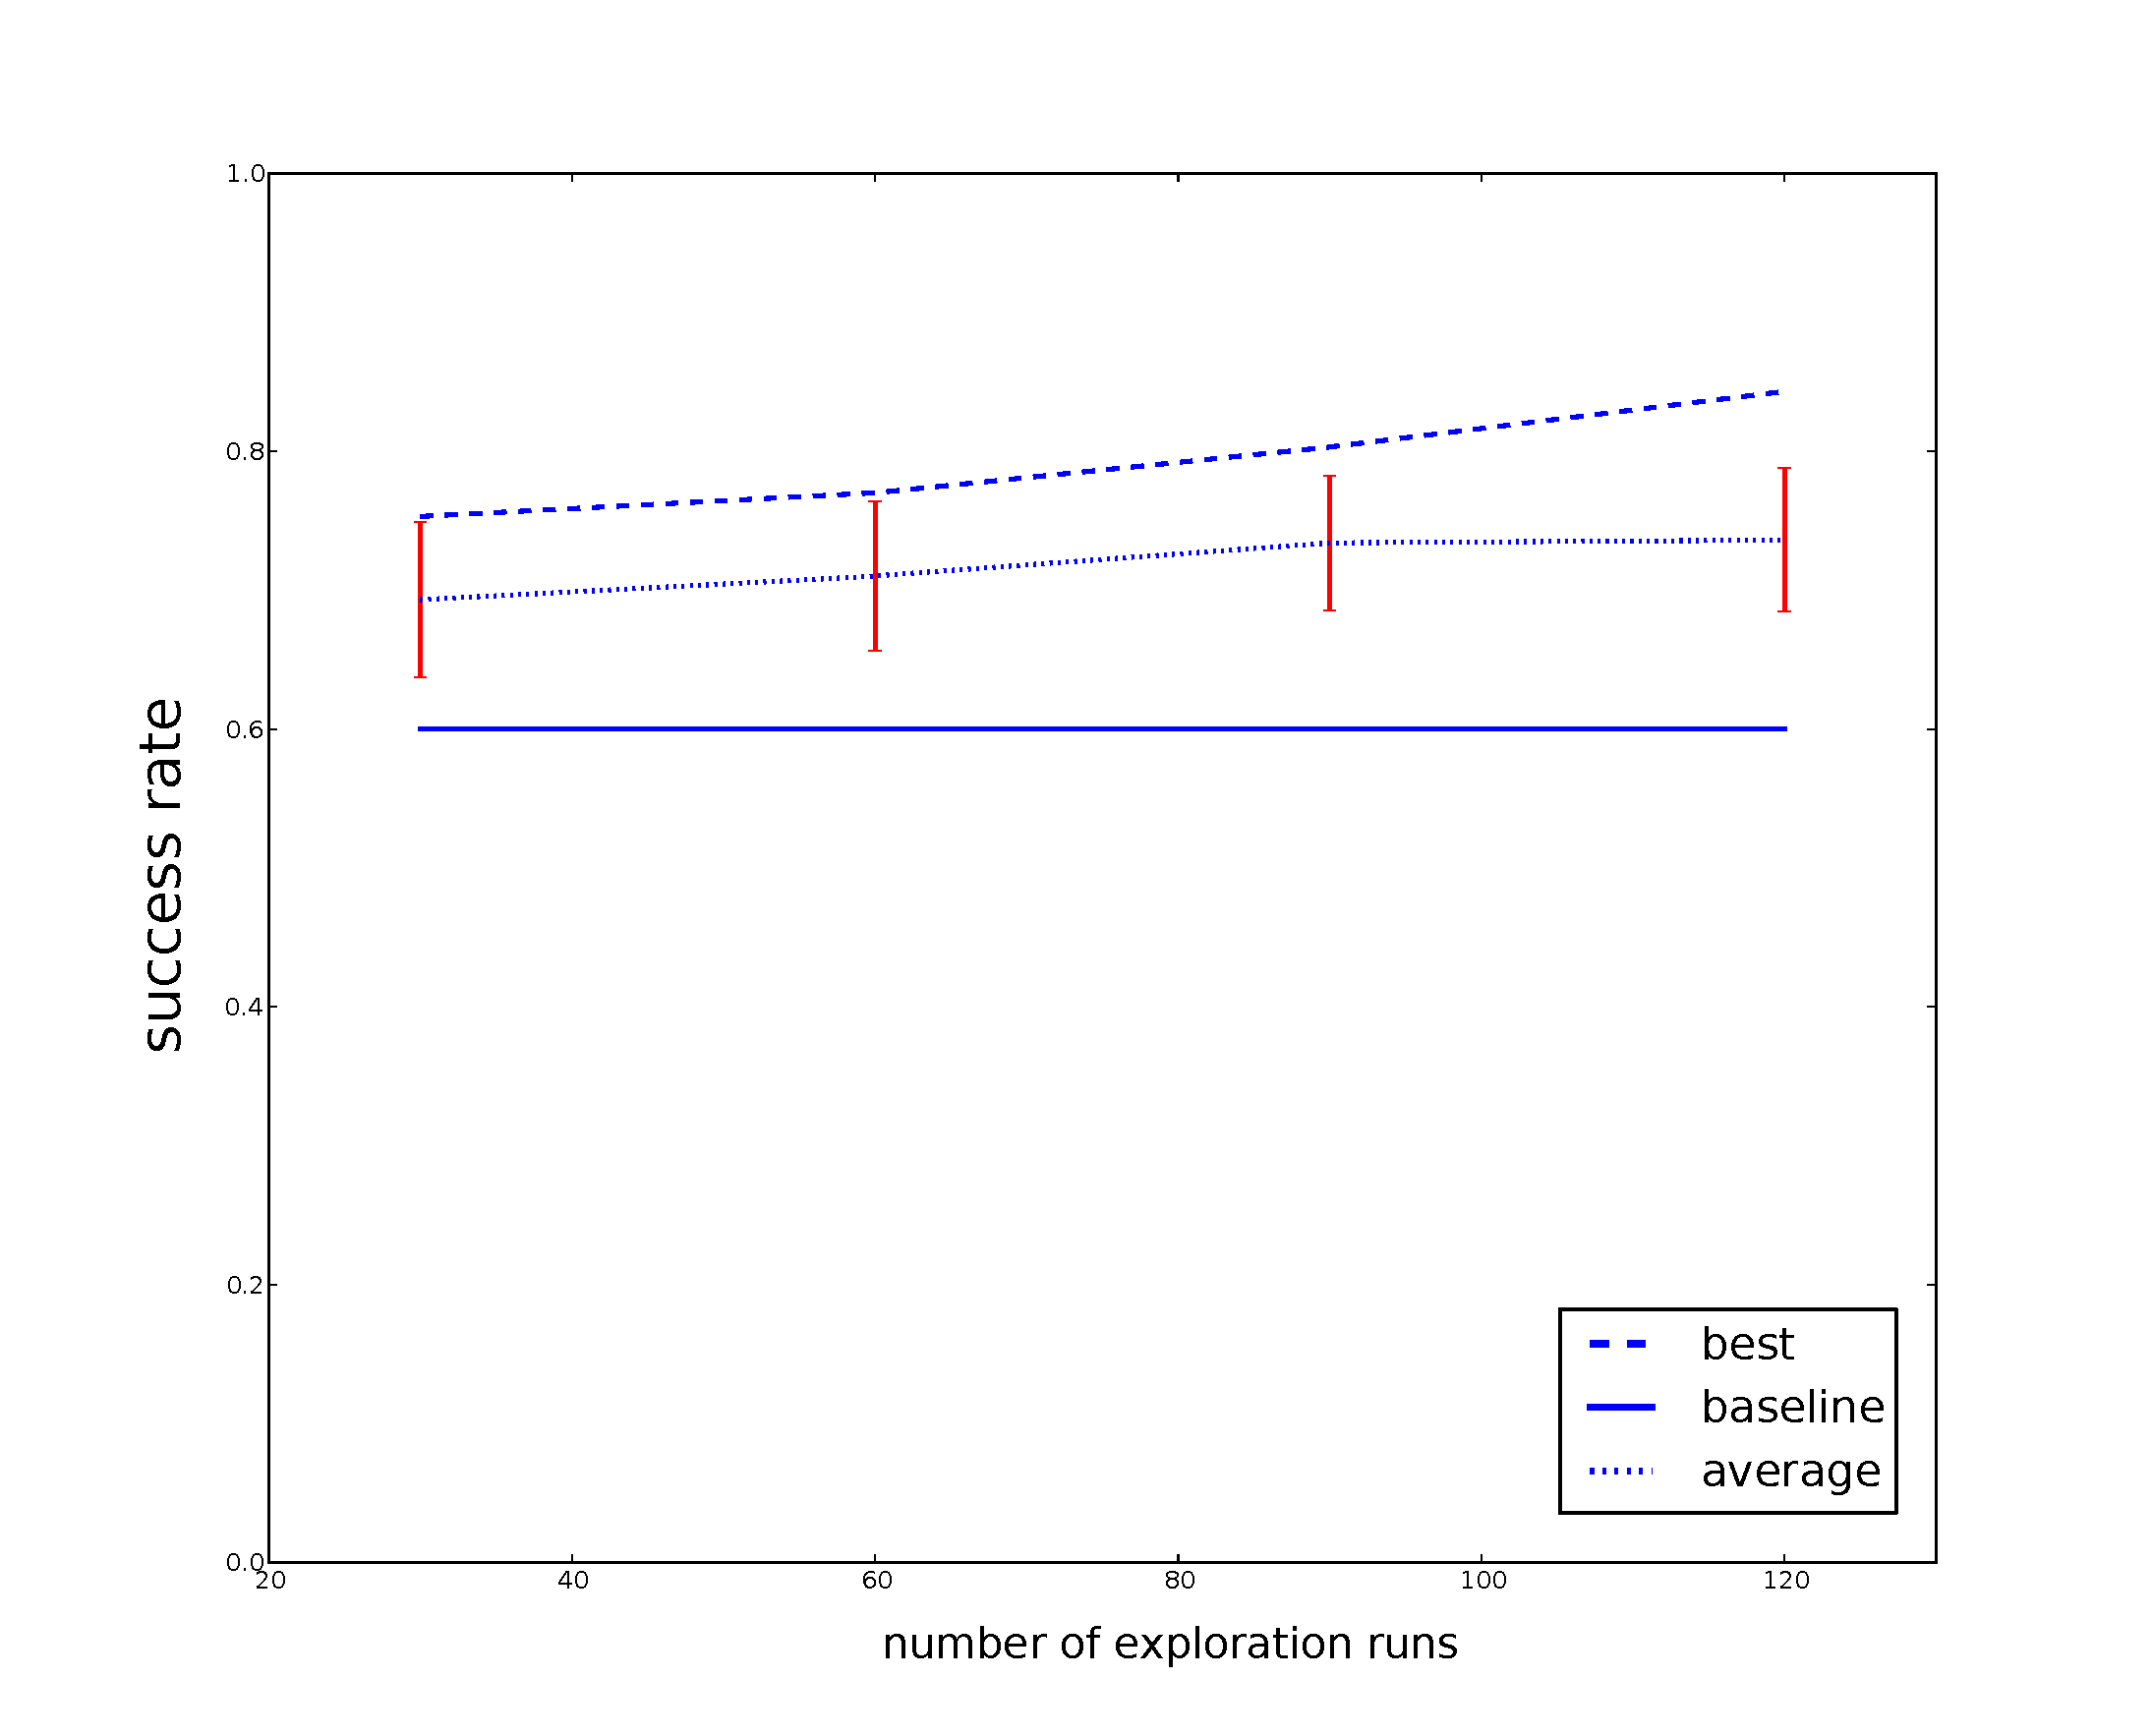
\includegraphics[width=\linewidth]{figs/results.pdf}
  \caption{Success rate of tying a an overhand knot in simulation with bootstrapped 
          examples compared with the baseline approach from Schulman et 
          al.~\cite{Schulmanetal_ISRR2013}. The problems for this scenario were generated
          by selecting a random initial state from a demonstration library and perturbed
          randomly by dragging random points on the rope. Directly transferring from the
          demonstrations achieves a success rate of 59\%. After doing 170 round of bootstrapping,
          we are able to improve on to an average of 74\% success. Our top performing trained set
          achieved 84\% success, an improvement of 25\% over the baseline. This success can
          be attributed to several factors, key among them are better modelling of states
          a trajectory can transfer to and ability to penalize less for deformations that 
          have allowed successful transfer in the past.}
  \label{fig:results}
\end{figure}

\begin{figure}
  \begin{subfigure}[b]{.48\linewidth}
    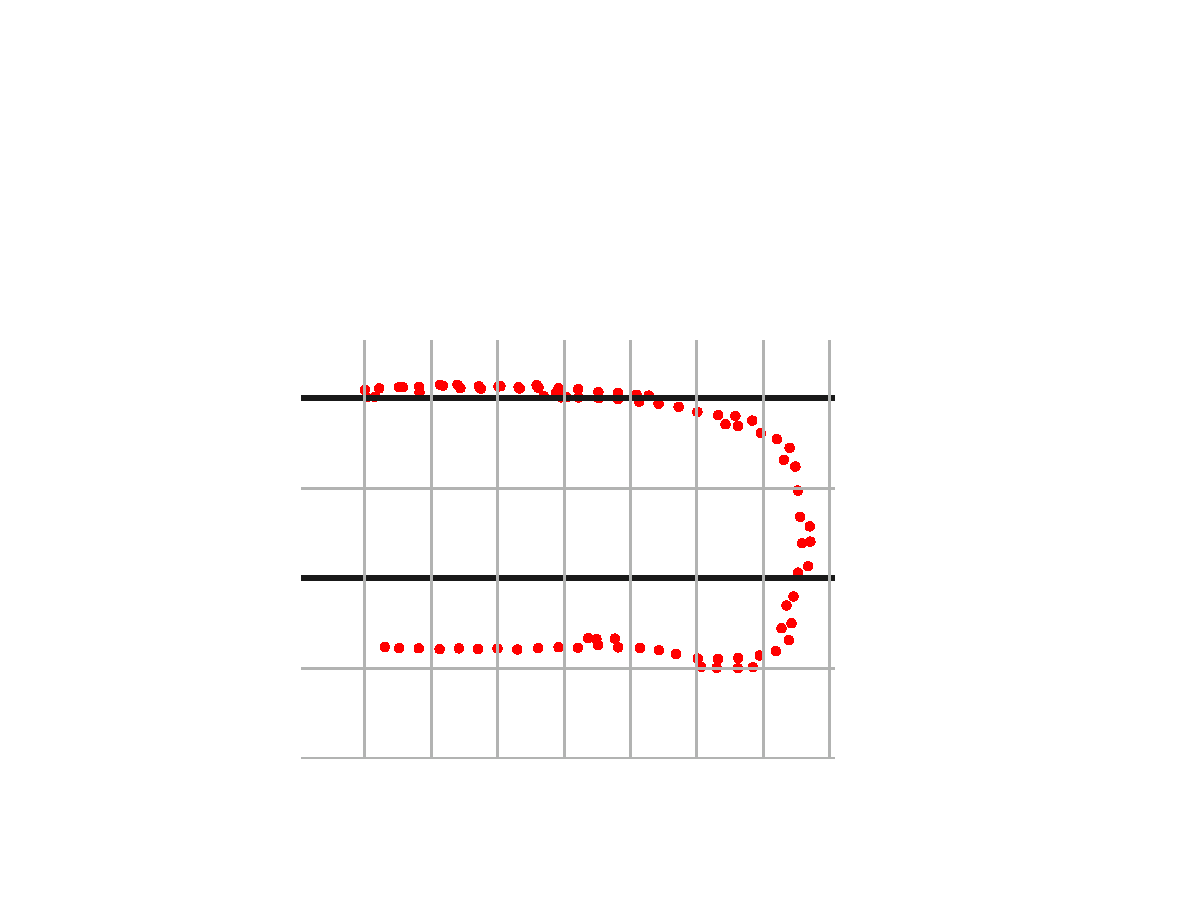
\includegraphics[width=\textwidth]{figs/orig.pdf}
    \caption{Original Segment}
    \label{fig:no_warp}
  \end{subfigure}
  \begin{subfigure}[b]{.48\linewidth}
    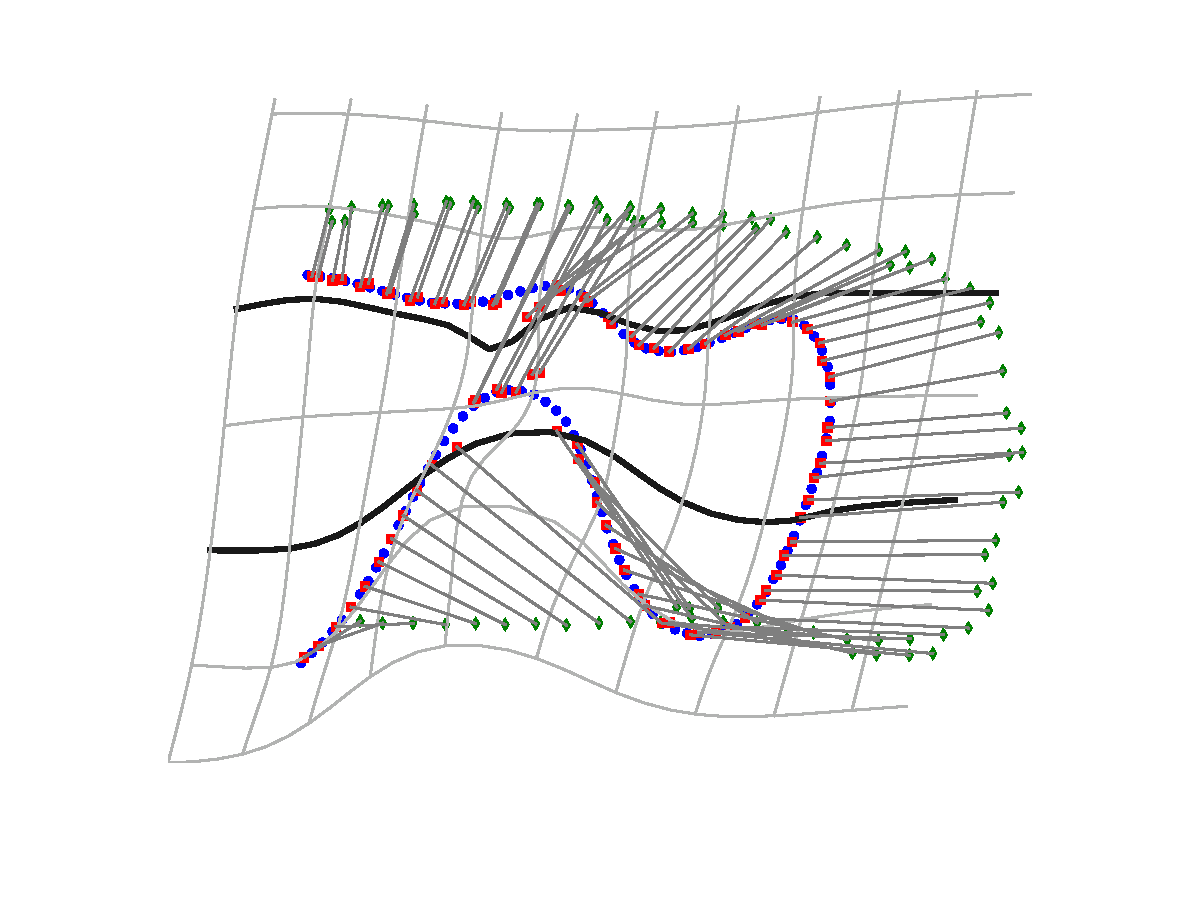
\includegraphics[width=\textwidth]{figs/warp_root.pdf}
    \caption{Directly Applying TPS-RPM}
    \label{fig:warp_root}
  \end{subfigure}
  \begin{subfigure}[b]{.48\linewidth}
    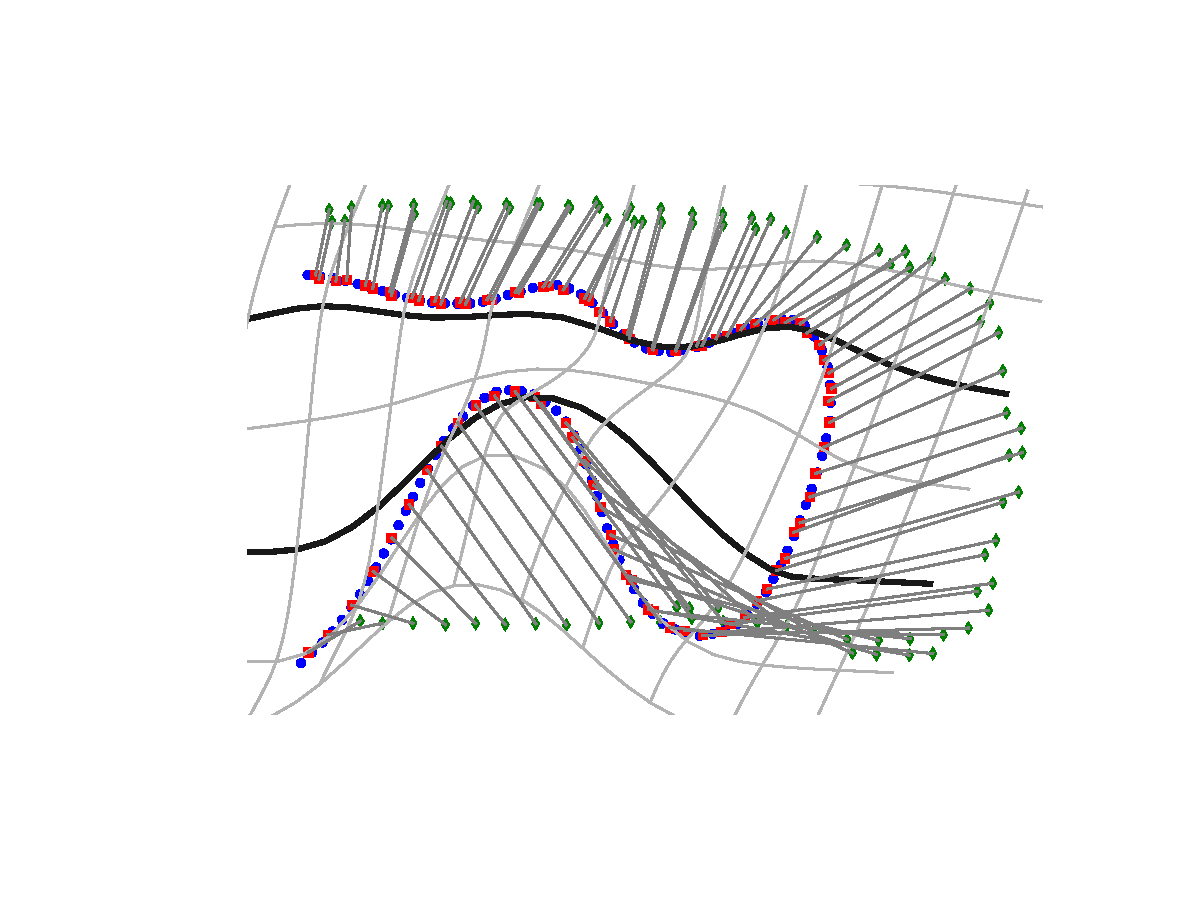
\includegraphics[width=\textwidth]{figs/warp_root_known.pdf}
    \caption{Known Correspondences}
    \label{fig:corresponds}
  \end{subfigure}
  \begin{subfigure}[b]{.48\linewidth}
    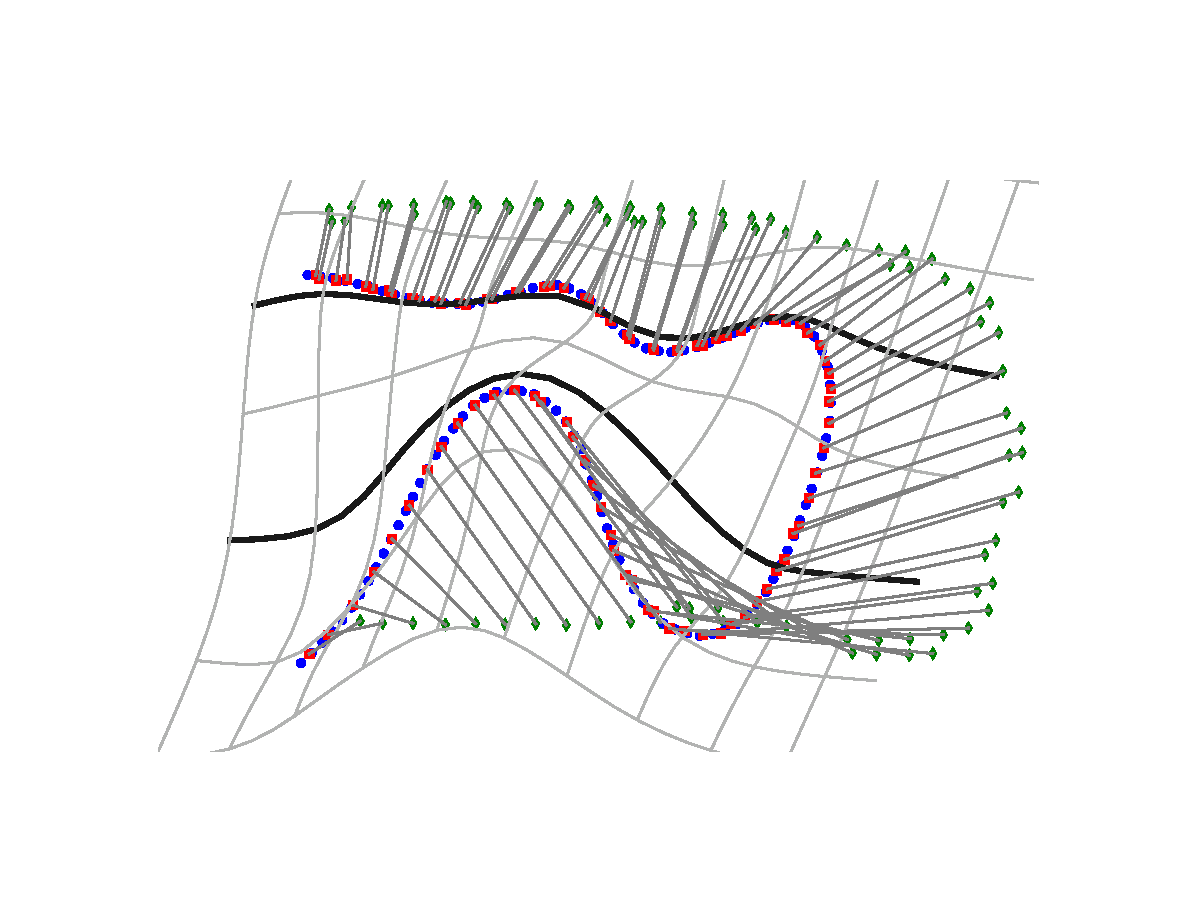
\includegraphics[width=\textwidth]{figs/warp_derived.pdf}
    \caption{Bootstrapping}
    \label{fig:bootstrap}
  \end{subfigure}
  \caption{Illustrations of various methods of Thin Plate Spline mappings.
  (a) shows the state from the demonstration being warped. (b) shows the results of directly warping from this state with TPS-RPM. The differences between the demonstration state and current state cause errors errors in the correspondences. (c) shows the results of directly fitting a thin plate spline with known correspondences. The intersection of the bold line and the rope (which are seperate in the initial scene) illustrates a large amount of non-rigidity in the $Z$-dimension to reduce the warping the X-Y plane. This can cause trajectory transfer to fail for this task. (d) shows the results of warping from a nearby bootstrapped state. The overall structure of the demonstration scene is better mapped into this scene because the iterated thin plate spline does not penalize for deformations that led to successful trajectory transfers during training.}
  \label{fig:warps}
\end{figure}



\section{Conclusion and Future Work}
\input{conclusion.tex}

\addtolength{\textheight}{-12cm}   % This command serves to balance the column lengths
                                  % on the last page of the document manually. It shortens
                                  % the textheight of the last page by a suitable amount.
                                  % This command does not take effect until the next page
                                  % so it should come on the page before the last. Make
                                  % sure that you do not shorten the textheight too much.

%%%%%%%%%%%%%%%%%%%%%%%%%%%%%%%%%%%%%%%%%%%%%%%%%%%%%%%%%%%%%%%%%%%%%%%%%%%%%%%%



%%%%%%%%%%%%%%%%%%%%%%%%%%%%%%%%%%%%%%%%%%%%%%%%%%%%%%%%%%%%%%%%%%%%%%%%%%%%%%%%



%%%%%%%%%%%%%%%%%%%%%%%%%%%%%%%%%%%%%%%%%%%%%%%%%%%%%%%%%%%%%%%%%%%%%%%%%%%%%%%%


\section*{APPENDIX}

Appendixes should appear before the acknowledgment.

\section*{ACKNOWLEDGMENT}

The preferred spelling of the word ÒacknowledgmentÓ in America is without an ÒeÓ after the ÒgÓ. Avoid the stilted expression, ÒOne of us (R. B. G.) thanks . . .Ó  Instead, try ÒR. B. G. thanksÓ. Put sponsor acknowledgments in the unnumbered footnote on the first page.



%%%%%%%%%%%%%%%%%%%%%%%%%%%%%%%%%%%%%%%%%%%%%%%%%%%%%%%%%%%%%%%%%%%%%%%%%%%%%%%%

References are important to the reader; therefore, each citation must be complete and correct. If at all possible, references should be commonly available publications.


\bibliographystyle{plain}
\bibliography{references}


\end{document}
               </include>
                </context>

                <context id="include" style-ref="include" class="no-spell-check">
                    <prefix>\\</prefix>

                    <keyword>input</keyword>
                    <keyword>include</keyword>
                    <keyword>includeonly</keyword>
                    <keyword>usepackage</keyword>
                </context>

                <context ref="common-commands"/>
                <context ref="specials-symbol"/>
                <context ref="command"/>
            </include>
        </context>
  </definitions>
</language>
